\chapter{Explaining Neural Networks}

This chapter provides an introduction to the growing field of explainable artificial intelligence.
We start with the motivation for understanding the decisions of neural networks and a brief overview of the legal obligations imposed on decision support systems by the European Union.
We continue with a review of several explainability methods suitable for our domain and task.
This will serve as a basis for the next chapter, where we evaluate selected methods against our benchmark.

In contemporary literature, several terms are used to address the incomprehensibility of ML models. Arrieta et al. \cite{arrieta-taxonomy} distinguish the following idioms:

\begin{enumerate}
    \item Understandability: Characteristic of a model to make a human understand its function without any need for explaining its internal structure or the algorithmic means by which the model processes data internally
    \item Comprehensibility: Ability of a learning algorithm to represent its learned knowledge in a human-understandable fashion 
    \item Interpretability: Ability to explain or to provide the meaning in understandable terms to a human.
    \item Explainability: An accurate proxy of the decision maker and comprehensible to humans.
    \item Transparency: A model is considered to be transparent if, by itself, it is understandable.
\end{enumerate}

In cite \cite{arrieta-taxonomy}, they further emphasize the distinction between interpretability and explainability -- interpretability, closely coupled with transparency, are inherent and passive properties of a machine learning model.
Explainability, on the other hand, is an initiated action taken to clarify the internal details of the models.
Both can be seen as means to achieve understandability -- how a human can make sense of decisions made by a model.


\section{Need for understandability}\label{sec:need-for-xai}

State-of-the-art neural network models are often products of billions of parameters \cite{arrieta-taxonomy}.
The term "black-box" models has been coined to highlight their complex internal mechanics.
In a crusade for ever greater performance and accuracy, models are inherently growing in size and depth.
According to \cite{arrieta-taxonomy, xai-survey}, this increasing size and complexity raises concerns in the research community and the general public about whether these networks can be trusted and used responsibly.

\subsection*{Spurious Correlations}

Distrust does not only stem from a lack of insight into the model's internal reasoning.
In some cases, the flawless performance of machine learning models may result from a systematic bias in training and evaluation data.
A common example is an experiment by Ribeiro et al. \cite{xai-husky}, where they deliberately trained a classifier to distinguish between wolves and huskies.
They constructed the dataset so that images of wolves consistently featured snow in the background, whereas images of huskies did not.
This led the classifier to base its decisions on the presence of snow in the image rather than the animal itself. 

\myref{Figure}{fig:horse-tag} presents a more unintentional example.
One can see that a \emph{capable} model can arrive at the desired output despite ignoring features on which humans would base their decision-making process. 

Examples like this show that the understandability of a decision support system is not just an issue for the end user.
It's also beneficial to the model's development cycle.
By gaining insight into the factors that influence the model's decisions, we can responsibly assess whether its reasoning matches our expectations --- and take action if it does not.

\begin{figure}[!h]
    \begin{center}
    \begin{minipage}{1\textwidth}
      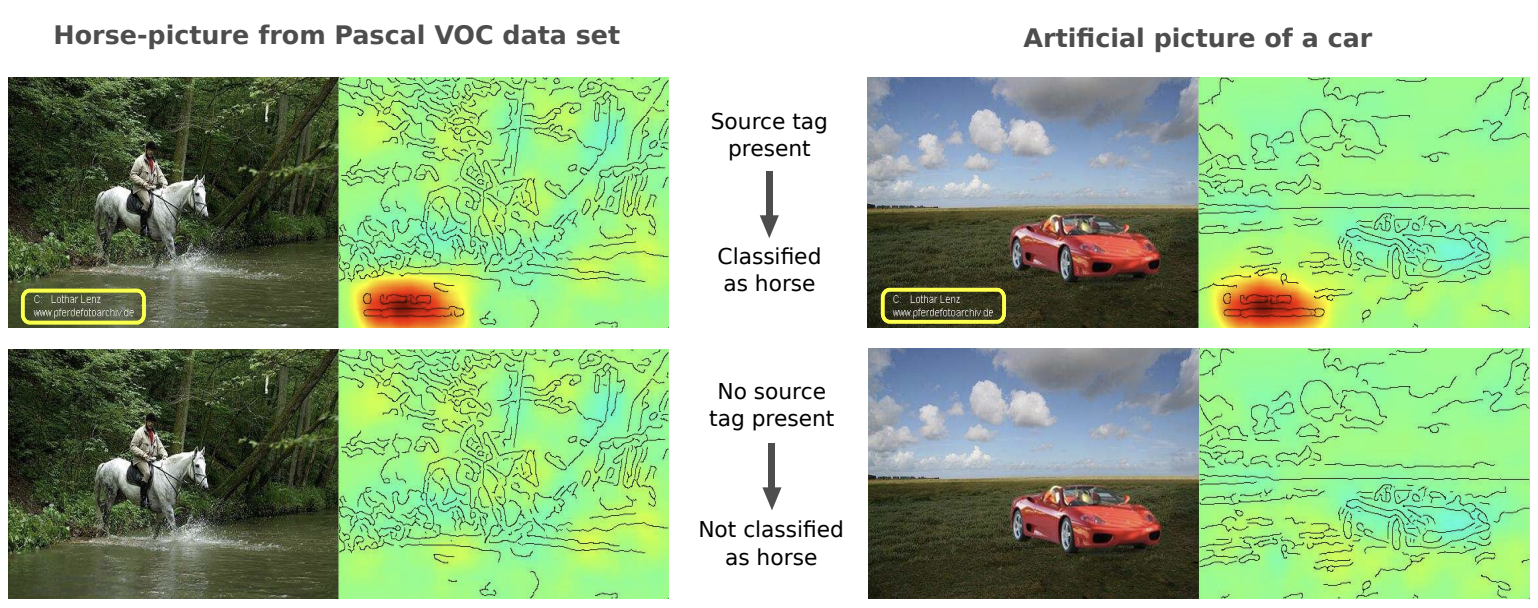
\includegraphics[width=\textwidth]{img/horse-tag.png}
    \end{minipage}
    \caption{Experiment conducted by Samek et al. \cite{xai-horse}. Their model was trained on the PASCAL-VOC dataset \cite{pascal-voc}. After the training, they found the presence of so-called \emph{spurious correlation}. Pictures of horses are classified solely on whether the bottom-left corner of an input image contains a source tag. If the source tag is manually added to an otherwise correctly classified image of a car --- the model changes its prediction, and the image is classified as a horse instead. Picture taken from \cite{xai-horse}.}
    \label{fig:horse-tag}
    \end{center}

\end{figure}

\subsection*{Explainability in medical domain}

Such spurious correlations and the black-box tag make clinicians skeptical about integrating DL models into healthcare.
A recent survey by GE HealthCare \cite{ge-healthcare-survey} concludes that of $2000$ clinicians who participated, $58$ percent do not have overall trust in artificial intelligence systems, and $44$ percent of respondents believe that the AI-based systems are biased.
Gaining the trust of both clinicians and patients is crucial to enabling industry-wide utilization of deep learning-based decision support systems.

\subsection*{Legal obligations for AI explainability in the European Union}

In certain contexts, understanding the model is not only a moral obligation.
In 2016, the European Union included the \emph{right to explanation} within the General Data Protection Regulation (GDPR).
Specifically, Articles 13 and 14 of the GDPR give individuals the right to receive ``meaningful information about the logic involved'' when they are a part of an automatic decision-making process.
This implies that we must take adequate measures to be able to explain decisions made by deep learning-based DSSs.
More on what Articles 13 and 14 mean for AI is to be found in a paper by Goodman and Flaxman \cite{xai-gdpr}.

Another piece of legislation from the European Union is anticipated to be implemented in May or June of 2024.
The \emph{AI Act} introduces a series of regulations for machine learning-based AI systems.
The legislation is notably more detailed and exhaustive than Articles 13 and 14 of the GDPR, yielding mixed responses from domain experts.
While the full implications are yet to be seen, it already imposes several restrictions on what must be met before deploying machine learning models.
One section of the legislation specifically targets high-risk AI systems.
It states that ``providers must build for human oversight, incorporating human-machine interface tools to ensure systems can be effectively overseen by natural persons.''.
Several aspects of the models' life-cycle are also revised, ranging from training datasets to technical documentation.
A comprehensive overview of the article is beyond the scope of this thesis and is summarized by Veale and Borgesius in \cite{xai-ai-act}.

\section{Explainable Artificial Intelligence}

The rapid development of deep learning models and scarcity of trust among users, combined with an attempted regulation, necessitate the development of tools and methods that allow us to understand and justify the outputs of otherwise opaque systems.
To shed light on the internal processes of machine learning models, a sub-field of Explainable Artificial Intelligence (XAI) covers a range of techniques to make models more understandable while preserving their performance and effectiveness.
XAI techniques enable humans to build trust and manage machine learning-based decision support systems, a crucial part of integrating systems based on deep learning.
The exact borders of the field are not firmly set, and the notion of what it means to explain a model is an ongoing matter of discussion \cite{xai-survey}.

In this thesis, the term `XAI' will refer to the subfield dedicated to advancing understandability in AI, and `explainable artificial intelligence' will denote the attribute of machine learning models that enables a certain level of understandability.
Arietta et al. \cite{arrieta-taxonomy} describe explainable artificial intelligence as follows: ``Given an audience, an explainable Artificial Intelligence is one that produces details or reasons to make its functioning clear or easy to understand.''.

The field of XAI distinguishes between two means of making artificial intelligence understandable:
\begin{enumerate}
    \item Using transparent model: Models based on linear regression or decision trees are inherently interpretable -- therefore understandable by themselves. We can derive how they came to the given conclusion by looking at their parameters.
    \item Using post-hoc explainability methods: When dealing with neural networks, we gain little insight into how they operate by simply inspecting their weights. Therefore, we must implement auxiliary methods, which simplify and distill the reasoning of networks so that, according to the definition --- we get a clear and easy-to-understand explanation. Post-hoc explainability methods can be further divided into two subgroups -- global methods explaining the model as a whole and local methods, which focus on internal reasoning behind prediction for a particular input sample.
\end{enumerate}

In recent years, a plethora of both global and local post-hoc explainability methods have been introduced to help grasp the decision process of deep neural networks.
According to the taxonomy proposed by Arietta et al. \cite{arrieta-taxonomy}, post-hoc methods can be further divided into two groups. 
Model-specific methods are designed to explain only models with specific features and capabilities -- such as attention-based models or convolutional neural networks.
Conversely, model-agnostic methods are capable of explaining arbitrary machine-learning models.

\section{Making CNN's Understandable}\label{sec:xai-cnn}
\todo{what is attribution}

For convolutional neural networks, the standard is to visually highlight parts of an image that are considered \emph{important} to the model.
The result of such visualization is commonly referred to as a saliency map, class activation map, or attribution map.
There is no consensus on terminology, and we will use the terms saliency map and explanation to describe any heatmap that identifies regions considered important by a post-hoc method.

The following subsections overview several explainability methods that we benchmark in \myref{Chapter}{experiment}.
We deliberately chose methods not covered in \cite{gallo}.
Methods such as LIME \cite{xai-husky}, Deconvolution \cite{deconvolution}, or $\epsilon$-LRP \cite{lrp}  were either computationally too expensive or produced sub-par results, which are not deemed satisfactory \cite{gallo}.
When choosing methods for this thesis, we focused on the observation of Gallo et al. \cite{gallo} --- methods, which tend to attribute continuous regions of tiles scored higher in the previous benchmarks.
Therefore, we focused on methods specifically created for explaining CNNs, leveraging their spatial memory ability, some of which were overviewed in \cite{krajnansky-grad-cam, bajger-grad-cam, hruska-grad-cam}.

\subsection{Occlusion}\label{occlusion}

Occlusion is a model-agnostic method from a family of so-called input perturbation-based methods.
Occlusion computes the saliency map by systematically covering square parts in the input image and observing the change in models' prediction confidence on the perturbed image.
Intuitively, we expect that when we cover (occlude) an important part of the input image, the confidence of our classifier drops.
On the contrary, when we cover a region without relevant features, the output should not differ too much from the output for the non-perturbed image.
The visual example can be seen in \myref{Figure}{fig:occ-saliency}. This approach gives us a rough (depending on the patch size) heatmap of input feature saliency.

An experiment conducted by Gallo et al. in \cite{gallo} shows that this method produces semantically correct saliency maps, recognizing morphological features indicating several Gleason patterns.
Sadly, Occlusion comes with high computational complexity and resource utilization.
For our use case, using an occlusion patch of $55 \times 55$ pixels and stride of $27$ pixels, the method needs 289 forward passes to compute the saliency map for a single tile.
On a machine with $8$ cores, $16$GB of RAM, and $48$GB of GPU memory capacity, occlusion needs approx. $2$ seconds and $40$GB of GPU memory to generate a single saliency map.
Recall \myref{Section}{sec:dataset} and our approach to WSI tiling.
In our test set, slide size varies from 400 to 4000 tiles per slide.
Omitting auxiliary saliency map processing, occlusion takes anywhere from $13$ to $130$ minutes to explain a single WSI.

\begin{figure}[!h]
    \begin{center}
    \begin{minipage}{1\textwidth}
      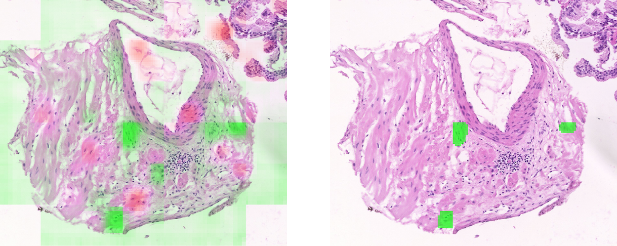
\includegraphics[width=\textwidth]{img/occlusion.png}
    \end{minipage}
    \caption{Sample of prostate tissue with Occlusion generated saliency. Green areas denote parts important for the model, while red parts signify non-cancerous areas. Since saliency maps are generated on a tile level, they are further composed, and overlapping areas are averaged to produce slide-level saliency maps. We apply the sigmoid function to saliency maps before combining, as is reported in \cite{gallo} to positively affect the smoothing and stability of the explanations. We do not use produced saliency maps as they are since they tend to be very noisy, as depicted in the left picture. Instead, the saliency map is thresholded to include only the most salient features, as depicted on the right, with a threshold of $55$ percent.}
    \label{fig:occ-saliency}
    \end{center}
\end{figure}

\subsection{CAM \& GradCAM}\label{subsec:cam}

Zhout et al. \cite{cam} show that introducing a GAP layer to a convolutional neural network has a welcome side-effect --- aside from regularization during training, it enhances network localization capabilities, despite being trained on image-level labels only --- without specifying where in the input the object of interest resides.
Their proposed method, called Class Activation Mapping (CAM), is used to visually highlight regions of input image used by the CNN to predict certain class $c$.
This model-specific method works only with networks with a GAP (or GMP) layer as the intermediate between the last convolutional layer and the final fully connected layer.
If a network satisfies this property, it is said to have a ``CAM architecture''.
The original paper uses a network with a convolutional layer before global pooling.
Our model features there a pooling layer instead.
This difference does not affect the results overviewed in the following paragraphs, and we will model them using a convolutional layer as per the original paper. 

Intuitively, CAM is a weighted sum of activation maps of the last convolutional layer.
Consider a network with convolutional layer with $K$ activation maps $A^1, A^2, \ldots, A^K$, followed by a GAP layer and a single fully connected layer.
In the fully connected layer, we fix neuron denoting class $c$, for which we want to compute a saliency map.
Recall \myref{Equation}{gap}, and that GAP reduces the value of each activation map $A^k$ to a single value $a^k$ --- the average of the activation map.
The score of the network for class $c$ is then calculated as
\begin{equation}\label{eq:gap-score}
    y^c = \sum_{k=1}^K w_{ck} a^k.
\end{equation}

To construct a CAM saliency map for class $c$, we reverse-engineer the calculation of $y^c$. The saliency map is constructed out of individual mappings, and mapping for spatial element $(S^c_{\text{CAM}})_{ij}$ is calculated as a weighted sum of activation maps $A^k$
\begin{equation}\label{eq:cam}
    (S^c_{\text{CAM}})_{ij} = \sum_{k=1}^K w_{ck}  A^k_{ij}.
\end{equation}
To obtain saliency map $S^c_{\text{CAM}}$, we calculate mappings for all pairs $i, j$.
The saliency map $S^c_{CAM}$ directly indicates the importance of the respective spatial locations.
If pooling layers are present in the network, they lead to the last convolutional layer having activation maps of smaller dimensions than the input grid.
This is addressed by up-sampling the $S^c_{\text{CAM}}$ to the size of the original input image.

The authors point out that this method is particularly useful for networks featuring the GAP layer.
They claim that using GMP instead leads to the method pointing out the single most discriminatory location instead of all of them, as is the case for GAP.
While this has been largely confirmed by their experiment on the ILSVRC dataset \cite{ilsvrc}, we believe that the method is worth considering for our use case.
Models employed in the experiment by Zhou et al. \cite{cam} are trained to distinguish between $1000$ classes, with their last convolutional layer having $1024$ units.
This configuration suggests a roughly one-to-one relationship between the pooled activations and the classes the network aims to identify.
In our setting, the last convolutional layer has $512$ units to identify one class --- we posit that even though we eventually only extract the most discriminative location from each activation map, having $512$ units should still yield robust localization performance.
Our belief is supported by the fact that upon inspection of the weights of the fully connected layer of the model described in \myref{Section}{model}, $267$ weights are positive --- meaning corresponding pooled activations are pro-cancerous.

Unlike CAM, GradCAM \cite{grad-cam} is a model-agnostic method that can explain various CNN architectures without needing a global pooling layer.
The idea is that since the convolutional layer holds spatial information about its activations, we can highlight the important ones using partial derivatives of the score $y^c$.

We will use the same setting as for \myref{Equation}{eq:cam}, with $L$ being a fixed convolutional layer of our network with $K$ units whose activation maps are $A^1, A^2, ..., A^K$.
GradCAM computes importance weight $i_{ck}$ for feature map $A^k$ as the average of partial derivatives of $y^c$ with respect to individual activations of $A^k$ \cite{grad-cam}
\begin{equation}\label{grad-cam-weights}
    i_{ck} = \frac{1}{|A^k|} \sum_{i=0}^H \sum_{j=0}^C \frac{\partial y^c}{\partial A^k_{ij}}.
\end{equation}

We substitute $i_{ck}$ for $w_{ck}$ in \myref{Equation}{eq:cam} and compute a weighted combination of activations and their respective importance to obtain a saliency map.
$\operatorname{ReLU}$ is applied over the weighted activations to get only positive values advocating for important features with respect to class $c$ \cite{grad-cam}
\begin{equation}\label{eq:gradcam-saliency-map}
    (S^c_{\text{GradCAM}})_{ij} = \operatorname{ReLU}\biggl(\sum_{k=1}^K i_{ck} A^k_{ij}\biggr).
\end{equation}
Authors of GradCAM took the inspiration for using $\relu$ from Deconvolution and Guided Backpropagation, both post-hoc methods already covered in \cite{gallo}.
In case the saliency map $S^c_{\text{GradCAM}}$ is smaller than the input grid, we up-sample it as in the case of $S^c_{\text{CAM}}$.

As shown in \cite{bajger-grad-cam}, for our model, GradCAM saliency maps are identical to the ones generated by CAM, up to a constant factor of ${1}/{|A^k|}$.
This consistency arises from our choice of GMP as the global pooling layer, which renders all partial derivatives zero, except for the derivative corresponding to the maximum activation in a given activation map $A^k$, which thus equals~$w_{ck}$.\looseness=-1

GradCAM has been previously covered in \cite{hruska-grad-cam, krajnansky-grad-cam, bajger-grad-cam}, but as far as we are concerned, this method was not evaluated using a quantitative benchmark similar to one from \cite{gallo}.
Since CAM produces saliency maps identical to GradCAM, we decided to include CAM in our benchmarks.

\subsection{GradCAM++}\label{sub:gradcampp}

GradCAM++ \cite{grad-cam-pp} is another gradient-based model-specific method to spatially attribute convolutional layer features for a given class.
Like GradCAM, this method leverages gradients flowing through the network to assess individual activations' importance while adressing several of GradCAMs' imperfections.

Chattopadhyay et al. \cite{grad-cam-pp} observed that if multiple occurrences of a class of interest $c$ are present in the input image, the localization capabilities of GradCAM worsen.
According to the authors, this stems from using unweighted partial derivatives in \myref{Equation}{grad-cam-weights}.
If there are multiple occurrences of class $c$, different feature maps may get activated, resulting in a diluted and faded saliency map.
They proposed a generalized solution that is equivalent in terms of computational performance.
First, they encode the importance weight $i_{ck}$ from \myref{Equation}{grad-cam-weights} as
\begin{equation}\label{eq:grad-cam-pp-weights}
    i_{ck} = \sum_i^H \sum_j^W \alpha^{ck}_{ij} \relu\biggl(\frac{\partial Y^c}{\partial A^k_{ij}}\biggr)
\end{equation}
adding a weight to each of the positive partial derivatives.
Here, $Y^c$ denotes the score $y^c$ put through the exponential function.

Then, they derive a method for expressing the partial derivative weights $a^{ck}_{ij}$ for all spatial locations in all activation maps.
They substitute weights from fully connected layer in \myref{Equation}{eq:gap-score} for importance weights $i_{ck}$ from \myref{Equation}{eq:grad-cam-pp-weights}, yielding
\begin{equation}\label{eq:grad-cam-pp-score}
    Y^c = \sum_{k=1}^K \biggl( \sum_{i=0}^H \sum_{j=0}^W \alpha^{ck}_{ij} \relu \bigl(\frac{\partial Y^c}{\partial A^k_{ij}}\bigr) \biggr) \biggl( \sum_{a=0}^H \sum_{b=0}^W A^{k}_{ab} \biggr)
\end{equation}
To express the weight $\alpha^{ck}_{ij}$, we need to take a partial derivative w.r.t. $A^k_{ij}$ twice. After that, we can rearrange the terms to obtain
\begin{equation}
    \alpha^{ck}_{ij} = \frac{\frac{\partial^2 Y^c}{(\partial A^k_{ij})^2}}{2\frac{\partial^2 Y^c}{(\partial A^k_{ij})^2} + \sum_{a=0}^H \sum_{b=0}^W A^{k}_{ab} \bigl( \frac{\partial^3 Y^c}{(\partial A^k_{ij})^3} \bigr)}.
\end{equation}

All that is left is to plug this expression back into \myref{Equation}{eq:grad-cam-pp-weights}.
This gives us the importance weights for activations, and the saliency map $S^c_{\text{GradCAM++}}$ is computed the same way as $S^c_{\text{GradCAM}}$.
Thanks to the additional coefficient $\alpha^{ck}_{ij}$ for respective partial derivative, authors claim that all spatial coordinates corresponding to instances of class $c$ in the input data will be highlighted with equal importance in the resulting saliency map.

As shown in \myref{Subsection}{subsec:cam}, two different methods can produce the same saliency map.
We derive the particular values for GradCAM++ importance weights $i_{ck}$ to avoid adding a third one.
The full derivative is presented in \myref{Section}{sec:grad-cam-plus-plus-weight-derivation} and yields
\begin{equation}
    i_{ck} = \frac{1}{2 + A^k_{ij}w_{ck}} \relu\bigl(\exp(y^c)w_{ck}\bigr)
\end{equation}
for $A^k_{ij}$ being the highest activation in activation map of unit $k$.

As a result, only activation maps corresponding to positive weights --- therefore, patterns detected as pro-cancerous --- are present in the final saliency map.
We lack rationale about the term $A^k_{ij} w_{ck}$ in the denominator, as more profound activations will receive a smaller importance weight.
Nevertheless, we have shown that for our architecture, GradCAM++ produces saliency maps that differ from CAM and GradCAM.
The extent to which the activation maps will differ hard to estimate, and we will include GradCAM++ in evaluation in \myref{Chapter}{experiment}.

\subsection{HiResCAM}\label{sub:hirescam}

HiResCAM, introduced in \cite{hires-cam}, is another gradient-based model-agnostic method that builds upon GradCAM's success.
The first step is the same as for GradCAM++ --- we need to compute partial derivatives of $y^c$ with respect to activation map $A^k$.
Instead of condensing the importance of the activation map to a single value, we arrange the partial derivatives into a grid and perform a pairwise multiplication of this grid with the respective activation map.
We compute the grid of partial derivatives for all activation maps $A^k$, and
\begin{equation}
    (S^c_{\text{HiResCAM}})_{ij}
        = \sum_{k=1}^K \frac{\partial y^c}{\partial A^k_{ij}} A^k_{ij}.
\end{equation}
The definition of the saliency map in \cite{hires-cam} omits the $\relu$, unlike GradCAM and GradCAM++.
However, in the implementation\footnote{\url{https://github.com/rachellea/hirescam}} corresponding to \cite{hires-cam}, the authors include the clipping and scaling --- therefore, HiResCAM saliency maps only include positive saliency.

Draelos and Carin \cite{hires-cam} arrived at a similar observation as in the case of GradCAM++ that GAP-ing the partial derivatives in \myref{Equation}{grad-cam-weights} leads to blurred feature maps. 
They believe that taking element-wise multiplication better reflects how models ``see" the input image.
This way, individual activations are scaled according to their partial derivative before being channel-wise summed up to form the final saliency map.

In addition to the method, the authors present proof of HiResCAM's capabilities.
The proof demonstrates that for convolutional networks ending in one fully connected layer $L$, HiResCAM guarantees to visually highlight all parts of the input image that increase class score $y^c$, given we compute the saliency map for the convolutional layer preceding $L$ \cite{hires-cam}.
Unfortunately, the proof does not cover our model introduced in \myref{Section}{model}.
While the model ends in one fully connected layer, it is separated from the last convolutional layer by an intermediate global max pooling operation, which reduces each feature map to a single value.
This breaks down the proof's assumption that we can extract spatial information from the feature maps in the FC layer, since such information will be destroyed in the GMP operation. 

The authors also show that given a model with CAM architecture employing GAP, saliency maps generated by HiResCAM collapse maps of the CAM method.
This does not hold for models using the GMP layer.
For our model, because of GMP, the partial derivative of $y^c$ with respect to $A^k_{ij}$ will be $w_{ck}$ iff $A^k_{ij}$ is the largest activation in $A^k$, and zero otherwise.
Therefore, we compose the resulting saliency map only from the most significant activations in each unit.
This differs from saliency maps produced by CAM and GradCAM++, which do not discriminate against individual activations that do not contribute to the model's output but are evidence for a detected pattern.
We believe that HiResCAM could better resemble how the Occlusion method produces the saliency maps since occluding features, albeit detected but not contributing to the output score because of GMP, should not produce a high saliency for the given region.

\subsection{ScoreCAM}

% \todo{add what is the baseline}
To bridge the gap between perturbation-based and gradient-based methods, Wang and Wang \cite{score-cam} introduced ScoreCAM to tackle GradCAM's flaws from different perspectives.
Unlike it is the case for previous CAM-based methods, ScoreCAM does not rely on partial derivatives to compute the saliency.
Instead, authors rely on a so-called increase in confidence, which is, given input $x$, baseline $x_b$, and activation $A^k$, defined as:
\begin{equation}
    c_k = f\bigl(x \odot \operatorname{upscale}(A^k)\bigr) - f(x_b)
\end{equation}
where $\operatorname{upscale}$ is a function that resizes activation map $A^k$ to the input grid size and scales it to range $[0, 1]$.
We get a score indicating how much network confidence changes if we only supply areas of the image where filter $F^k$ found a pattern it is trained to detect.
We calculate the final saliency map $S^c_{\text{ScoreCAM}}$ using the respective increases in confidence $c_1, \ldots, c_K$ as importance weights for the $K$ activation maps of layer of interest, replacing corresponding $i_{c1}, \ldots, i_{cK}$ in \myref{Equation}{eq:gradcam-saliency-map}.

\subsection{AblationCAM}

Another gradient-free method, AblationCAM, introduced in \cite{ablation-cam}, utilizes ablation analysis to compute the importance of activation maps.
AblationCAM computes how an individual activation map $A^k$ contributes to the final score $y^c$ by "removing" it from the score computation and observing a drop in the model's confidence.
The influence of the removal of activation map $A^k$ to the final score is defined as
\begin{equation}\label{eq:ablation-cam-importance-weight}
    d_{ck} = \frac{y^c - y^c_k}{y^c} = \frac{w_{ck}a^k}{y^c}
\end{equation}
where $y^c_k$ represents an output of the model, for which the activation $A^k$ is zeroed out.

Similar to Occlusion and input features, if we remove activations important to the network when assessing the presence of class $c$, the score $y^c$ should drop. To obtain the final saliency map, we compute the ablation weights for the layer of interest and substitute them instead of importance weights into \myref{Equation}{eq:gradcam-saliency-map}.

The globally pooled activations in the ablation weights could better distribute the saliency across the WSI once the tile-level explanations are combined, as not only the weight but also the strength of activations is taken into account.
However, we believe this effect is counteracted by the model's confidence $y^c$ in the denominator, which is inversely proportional to individual ablation weights.

\subsection{Layer-Wise Relevance Propagation}

While Occlusion estimated feature importance by observing changes in output and CAM-based methods utilized spatial information in the convolutional layers, Layer-Wise Relevance Propagation (LRP) \cite{lrp} takes a different approach.
Given an output score of the network, LRP utilizes several types of propagation rules to redistribute the score from the output layer down to the input pixels.
The idea is that we can look at how individual features contribute to the output of the network --- each feature value is weighted and sent to the upper layer across the whole network, ultimately contributing to the final class score.
In a reverse fashion, we can compute the importance of the input pixels \cite{lrp}.

To describe this procedure, assume that $i$ and $j$ are two neurons in consecutive layers, so there is a connection from $i$ to $j$. 
The process of propagating relevance $R_j$ from $j$ to $i$ is captured by the following generic propagation rule \cite{lrp}
\begin{equation}
    R_i = \sum_j \frac{z_{ji}}{\sum_k z_{jk}} R_j
\end{equation}
where $z_{ij}$ models to which extent neuron $i$ contributed to neuron $j$'s activation.
The extent $z_{ij}$ is derived by various rules, further described in \cite{lrp}.
The choice of rules is largely left to experimentation.
However, Montavon et al. \cite{lrp} provide a blueprint for choosing layers when working with a VGG-16-based network.

The main building block is the LRP-$0$ rule, where the extent
\begin{equation}
    z_{ji} = y_i w_{ji}.
\end{equation}
Parameters $y_j$ and $w_{ji}$ stand for neurons output and weight, respectively, as defined in \myref{Section}{section:dl}.
% \todo{are those really parameters?}

According to the observation of Montavon et al. \cite{lrp}, using solely LRP-$0$ leads to very noisy explanations.
To tackle the noise, we add a small positive term $\epsilon$ to the denominator --- $\epsilon$ will absorb weak and contradictory contributions, preserving only the salient scores. 
As a result, we typically get less noisy explanations.
Gallo et al. used the LRP-$\epsilon$ rule exclusively in \cite{gallo}.
However, such explanations were still deemed scattered and noisy.
To further enhance produced explanations, we can use the LRP-$\gamma$ rule to favor positive contributions by using a coefficient applied only to the positive weights:
\begin{equation}
    z_{ji} = {a_j \cdot (w_{ji} \cdot \gamma w_{ji}^+)}.
\end{equation}
The $\gamma$ rule draws from the LRP-$\epsilon$ rule and keeps the $\epsilon$ term in the denominator.
Figure \ref{fig:lrp-montavon} shows how multiple rules can be composed to visually enhance explanations.

\begin{figure}[!h]
    \begin{center}
    \begin{minipage}{1\textwidth}
      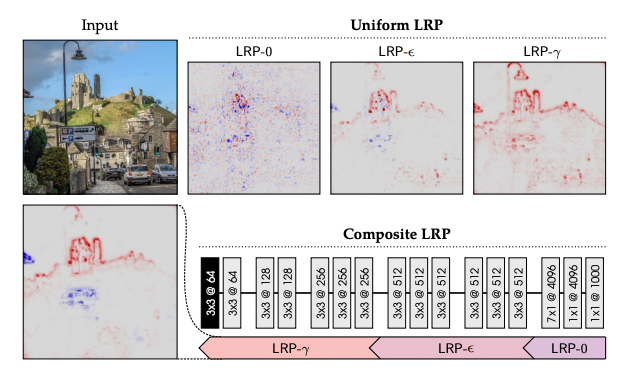
\includegraphics[width=\textwidth]{img/lrp-montavon.png}
    \end{minipage}
    \caption{Image show explanation results after different combinations of rules are applied. Notice that combining multiple rules yields a visually more coherent saliency map. According to Montavon et al. \cite{lrp}, using LRP-$0$ in the upper layers is beneficial to combat the entanglement of different concepts represented by the network. LRP-$\epsilon$ in the middle layer helps to propagate only the most salient activations, while LRP-$\gamma$ in the lower layer ensures uniform relevance spread. Image taken from \cite{lrp}.}
    \label{fig:lrp-montavon}
    \end{center}
\end{figure}